\chapter{DISCUSSION AND EVALUATION}

Three threads run through this chapter: a quantitative evaluation of the anomaly detection model, a cross-dimension analysis of system performance, and a mapping of the findings back to the three research questions from Chapter~1.

% ─────────────────────────────────────────────────────────────
\section{Anomaly Detection Model Evaluation}
\label{sec:ml_validation}

\subsection{Training Dataset Composition}

Table~\ref{tab:train_composition} lists all data used in the anomaly
detection pipeline, broken down by split and source.

The clinical data comes from the UCI Heart Disease Dataset~\cite{UCIHeartDisease1988}, a Kaggle release described as pooling records from four hospital sites (Cleveland, Hungary, Switzerland, VA~Long~Beach) totalling 1\,025 rows. Running \texttt{pandas.DataFrame.duplicated()} revealed that 723 of those rows are identical copies, leaving only 302 truly distinct records --- suggesting the multi-site collection largely replicates the well-known 303-patient Cleveland cohort rather than adding independent observations. The training pipeline does not apply explicit deduplication, so the 499 target=0 (healthy) rows drawn from the full CSV are used as-is; the duplicate Cleveland records therefore appear multiple times in training and inflate the effective weight of that cohort. This is acknowledged as a data-quality limitation in Section~\ref{sec:discussion_limitations}.

A second constraint is that the dataset records \texttt{thalach} --- peak HR achieved during a treadmill stress test --- rather than resting HR. Resting HR was approximated by scaling: $\texttt{thalach} \times \mathcal{U}(0.55,\,0.65)$, drawing the factor uniformly from $[0.55,\,0.65]$ to bring exercise-peak values into a plausible resting range. The scaling has no clinical basis and is the primary acknowledged limitation of this dataset; see Section~\ref{sec:discussion_limitations}.

The 1\,700 synthetic samples were added specifically to address a gap this conversion leaves open. Because all UCI readings originate from a supervised exercise protocol, none of them capture the lower HR values normal for an elderly person asleep at night (roughly 50--74\,bpm). Without these samples, early testing showed the model flagging normal sleep-time bradycardia as anomalies, so the synthetic night-time readings were added to push the decision boundary to a more realistic lower edge.

\begin{table}[H]
\centering
\caption[Data sources for the anomaly detection pipeline]{Data sources for the heart-rate anomaly detection pipeline.
  \emph{Production model} (\texttt{tune\_and\_retrain\_anomaly.py}) uses all data in the
  Production column; the \emph{Evaluation benchmark} (\texttt{benchmark/anomaly/eval\_benchmark\_model.py})
  uses only the UCI 80/20 split with no synthetic samples.}
\label{tab:train_composition}
\footnotesize
\setlength{\tabcolsep}{5pt}
\renewcommand{\arraystretch}{1.3}
\begin{tabular}{@{}
  l
  >{\raggedright\arraybackslash}p{3.2cm}
  r
  r
  >{\raggedright\arraybackslash}p{5.4cm}
@{}}
\toprule
\textbf{Split} & \textbf{Source} & \textbf{Samples} & \textbf{HR (bpm)} & \textbf{Notes} \\
\midrule
\multicolumn{5}{@{}l}{\textit{Production model training (contamination\,=\,0.020, $n\_estimators$\,=\,300)}} \\[2pt]
Train
  & Generated (code)
  & 1\,700 & 50--91
  & Night: 50--74\,bpm; daytime: 60--91\,bpm.
    Covers sleep-time HR absent from UCI. \\[3pt]
  & UCI healthy (target\,=\,0) \cite{UCIHeartDisease1988}
  & 499 & 40--123
  & All healthy records; resting HR estimated as
    $\texttt{thalach} \times \mathcal{U}(0.55,0.65)$. \\
\cmidrule(l){2-5}
  & \textbf{Production total} & \textbf{2\,199} & & \\
\midrule
\multicolumn{5}{@{}l}{\textit{Evaluation benchmark (80/20 UCI split, contamination\,=\,0.10, $n\_estimators$\,=\,200)}} \\[2pt]
Train
  & UCI healthy 80\,\% \cite{UCIHeartDisease1988}
  & 399 & 40--123
  & Same thalach estimation; no synthetic data used. \\[3pt]
Test
  & UCI healthy held-out 20\,\%
  & 100 & 40--123
  & Labelled \emph{normal}. \\[3pt]
  & UCI diseased (target\,=\,1) \cite{UCIHeartDisease1988}
  & 526 & varies
  & $\texttt{thalach} \times \mathcal{U}(1.10,1.25)$;
    labelled \emph{anomaly}. \\
\cmidrule(l){2-5}
  & \textbf{Eval test total} & \textbf{626} & & \\
\bottomrule
\end{tabular}
\end{table}

Figure~\ref{fig:if_eval_flow} summarises the end-to-end data flow of this
benchmark, from the raw UCI and synthetic sources through the 80/20 split and
contamination selection to the final evaluation on the shared held-out test set.

\begin{figure}[H]
\centering
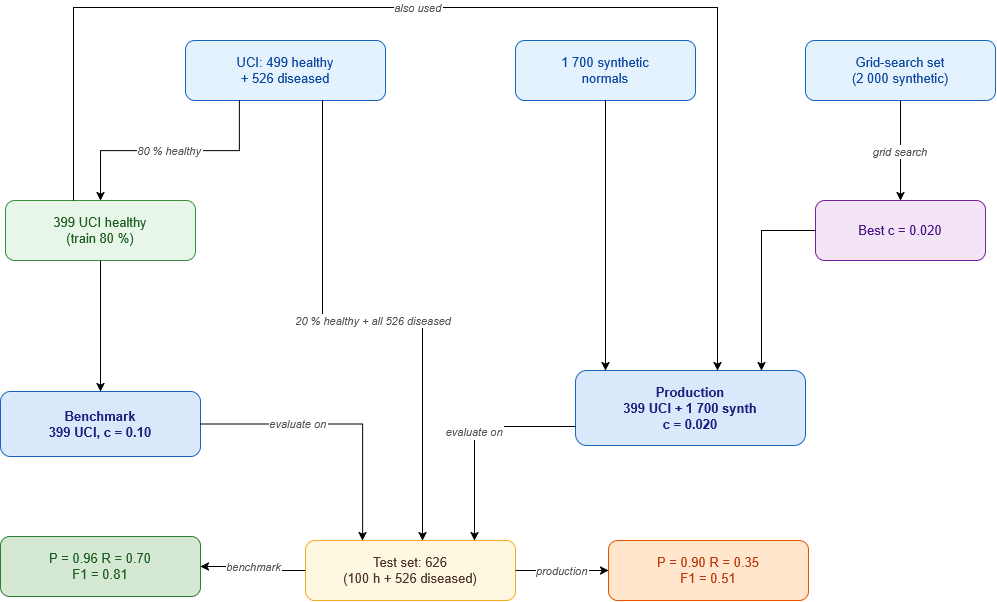
\includegraphics[width=0.95\textwidth]{images/fig_if_eval_pipeline.png}
\caption[Isolation Forest evaluation pipeline]{Isolation Forest training and evaluation pipeline.
\textbf{Row~1}: raw data sources.
\textbf{Row~2}: UCI is split 80/20 --- 399 healthy records go to training; 100 held-out healthy records plus all 526 diseased records form the 626-patient test set; the grid search selects contamination~=~0.020 on a separate 2\,000-sample synthetic set.
\textbf{Row~3}: two model configurations trained independently on different data and contamination settings.
\textbf{Row~4}: both models are evaluated on the same held-out test set; different contamination thresholds produce the differing precision/recall trade-offs.}
\label{fig:if_eval_flow}
\end{figure}

\subsection{Held-Out Evaluation}

Two contamination values are used. For the UCI held-out benchmark, \texttt{contamination}~=~0.10 is used in \texttt{eval\_benchmark\_model.py}, which trains a fresh Isolation Forest on 399 UCI healthy records (80\,\% split, no synthetic data, \texttt{n\_estimators}=200) and evaluates on the held-out test set, giving the reported metrics (P\,0.96, R\,0.70, F1\,0.81). For the production model, \texttt{contamination}~=~0.020 is chosen by grid search over the synthetic-plus-UCI training set (Section~\ref{subsec:synth_data}), tuned for a lower false-positive rate in continuous home monitoring. Both models use heart rate as the sole input feature.

The UCI held-out test set consists of 100 healthy records (20\,\% of the 499
UCI healthy records) and all 526 diseased records ($n=626$ total).
BPM values are approximated from UCI \texttt{thalach} (maximum exercise HR):
healthy records use $\texttt{thalach} \times \mathcal{U}(0.55, 0.65)$;
diseased records apply an additional upward factor
$\times\,\mathcal{U}(1.10, 1.25)$ to reflect elevated cardiac load.
The benchmark heart-rate-only Isolation Forest is evaluated on this set
(contamination~=~0.10); its anomaly-class metrics are shown in
Table~\ref{tab:ml_eval} and its confusion matrix in Table~\ref{tab:confusion}.

\begin{table}[H]
\centering
\caption[Anomaly-class evaluation: benchmark HR-only model]{Anomaly-class evaluation on the UCI held-out test set ($n=626$, contamination~=~0.10): benchmark heart-rate-only Isolation Forest}
\label{tab:ml_eval}
\small
\begin{tabular}{lcccc}
\toprule
\textbf{Model}  & \textbf{Precision} & \textbf{Recall} & \textbf{F1-Score} & \textbf{Support} \\
\midrule
Isolation Forest --- HR-only (benchmark)  & 0.96 & 0.70 & 0.81 & 526 \\
\bottomrule
\end{tabular}
\end{table}

\begin{table}[H]
\centering
\caption[Confusion matrix: benchmark HR-only model]{Confusion matrix on the UCI held-out test set ($n=626$): benchmark heart-rate-only Isolation Forest}
\label{tab:confusion}
\small
\centering
\begin{tabular}{llcc}
\toprule
 & & \multicolumn{2}{c}{\textbf{Predicted}} \\
 & & Normal & Anomaly \\
\midrule
\multirow{2}{*}{\textbf{Actual}}
  & Normal  & 86  & 14 \\
  & Anomaly & 159 & 367 \\
\bottomrule
\end{tabular}
\end{table}
\FloatBarrier

The benchmark heart-rate-only model achieves an F1-score of 0.81 for the anomaly class, with a precision of 0.96 and recall of 0.70 (detects 367/526 cases, with 14 false positives out of 100 healthy test records). The anomaly detector is intentionally designed as a single-feature model: only heart rate is a direct cardiac signal, so adding unrelated environmental features (room temperature, humidity, light level, time of day) would dilute the cardiac signal rather than improve detection. Formal definitions of the metrics are given in Appendix~\ref{app:ml_metrics}. A comparison against a simple threshold baseline is in Section~\ref{subsec:ablation}.

\subsection{Threshold Baseline Comparison}
\label{subsec:ablation}

Table~\ref{tab:feature_ablation} compares Isolation Forest with a rule-based threshold baseline (BPM $<$ 50 or $\geq$ 100) on the same UCI held-out test set. The threshold baseline performs better (F1=0.87), which is expected since the UCI cohort contains cardiac patients whose BPMs often fall outside the normal resting range. However, a fixed threshold is not adaptable to continuous home monitoring and cannot discriminate contextual anomalies from permanently elevated resting HR.

The Isolation Forest sacrifices some recall for a lower false-positive rate (precision 0.96 vs. 0.97), which is preferable in a home environment where alert fatigue is a practical concern. Crucially, these are not competing alternatives: the threshold is the deterministic first layer of the hybrid pipeline, while the Isolation Forest provides contextual detection for borderline readings --- see \emph{Reconciling recall} below.

\begin{table}[H]
\centering
\caption[Threshold baseline vs.\ Isolation Forest configurations]{Threshold baseline versus Isolation Forest configurations on UCI held-out test set ($n=626$). \textbf{Note: the two IF rows use different contamination values by design and are not directly comparable with each other} --- the benchmark uses $c=0.10$ to maximise F1 on UCI data; the production model uses $c=0.020$ to minimise false alarms in continuous home monitoring. Each IF row is compared independently against the threshold baseline.}
\label{tab:feature_ablation}
\small
\setlength{\tabcolsep}{5pt}
\begin{tabularx}{\textwidth}{@{} >{\RaggedRight\arraybackslash}X c c c c >{\RaggedRight\arraybackslash}X @{}}
\toprule
\textbf{Method} & \textbf{Contam.} & \textbf{Precision} & \textbf{Recall} & \textbf{F1} & \textbf{Purpose} \\
\midrule
Threshold baseline (BPM\,$<$\,50 or $\geq$\,100) & --- & 0.97 & 0.78 & 0.87 & Deterministic first layer; no training required \\
IF --- benchmark (UCI-only, 399 healthy, $n_\text{est}$=200) & 0.10 & 0.96 & 0.70 & 0.81 & Clean evaluation on real UCI data; source of headline metrics \\
IF --- production (UCI+synthetic, 2\,099 train, $n_\text{est}$=300) & 0.020 & 0.90 & 0.35 & 0.51 & Calibrated for low false-alarm rate; not optimised for UCI recall \\
\bottomrule
\end{tabularx}

\vspace{2pt}
{\footnotesize\RaggedRight\noindent
UCI held-out: 100 healthy + 526 diseased ($n=626$); BPM approximated from \texttt{thalach} ($\times$0.55--0.65).
Production IF uses 399 UCI-healthy for training (not 499) to keep 100 healthy test records unseen.
F1 values are computed from unrounded P and R before display rounding; threshold baseline raw F1 = 0.865, production IF raw F1 = 0.504.\par}
\end{table}

\paragraph{Reconciling recall with the safety requirement.}
Appendix~\ref{app:ml_metrics} notes that in a health-monitoring setting, recall (minimising missed anomalies) is the safety-critical metric. The benchmark recall of 0.70 appears to conflict with this, but the deployed system is a \emph{hybrid}, not a pure Isolation Forest: extreme readings are caught by hard clinical thresholds \emph{regardless} of the IF score (BPM\,$<$\,50 always triggers Caution; BPM\,$\geq$\,100 always triggers Warning or Critical — see Table~\ref{tab:risk}). The IF score is added only for contextual borderline readings in the 50--59 and 96--99\,bpm zones that the threshold alone would miss. The benchmark recall therefore describes IF in isolation on an all-or-nothing test; the system's effective recall for clinically extreme events is higher because those events are always caught by the threshold layer. The gap left unaddressed is contextual anomalies within the normal BPM band, which would require a per-patient baseline — an identified future-work item.

\subsection{Validation Limitations}
\label{sec:discussion_limitations}

Four limitations apply to this evaluation:

\begin{enumerate}

\item \textbf{Synthetic training samples.} There is no public dataset that provides labelled resting HR for elderly with timestamps. A set of 1,700 HR values was generated to model circadian variation (sleep: 50--74\,bpm, daytime: 60--91\,bpm), since using only the 499 UCI healthy samples would under-represent night-time resting HR and lead to over-flagging of normal bradycardia. 
Future work: replace them with actual elderly resting HR (e.g., PhysioNet MIMIC-IV).

\item \textbf{BPM estimation.} UCI provides max exercise HR (\texttt{thalach}), not resting HR. BPM is estimated as $\text{BPM} = \texttt{thalach} \times \mathcal{U}(0.55, 0.65)$ with an additional upward factor for diseased patients, adding noise that may blur healthy/diseased separation.

\item \textbf{Independent evaluation.} Readings are scored without regard to temporal context. Sequential models (LSTM, sliding windows) could exploit inter-reading correlations to reduce false negatives.

\item \textbf{Dataset duplication and leakage.} The UCI CSV holds 1\,025 rows but only 302 are distinct; the other 723 are exact copies, mostly of the Cleveland cohort. Because the pipeline trains on the full file without deduplication, an 80/20 split can place copies of the same record on both sides of the train/test boundary, which likely inflates the benchmark precision. Deduplicating before the split, or sourcing genuinely independent multi-site records, is identified as future work.

\end{enumerate}

The evaluation follows the same rationale as Suryadevara et al.~\cite{Suryadevara2012}
and Stolojescu-Crisan et al.~\cite{Stolojescu2021}, who validate against real
deployment data. The benchmark heart-rate-only model (F1\,=\,0.81) is evaluated
exclusively on real UCI clinical data.

% ─────────────────────────────────────────────────────────────
\section{System Performance Analysis}
\label{sec:performance}

\subsection{Command Latency Benchmark}
\label{subsec:latency_protocol}

A device toggle request goes from the client to the Flask backend, then over TLS through the EMQX Cloud broker, and finally to the ESP32. Latency here is reported as a 10-trial measurement on a single session; a full 30-trial campaign across different network conditions is planned for post-defence work (Section~\ref{sec:future}).

Table~\ref{tab:latency_record} reports a 10-trial HTTP command dispatch
measurement using \texttt{benchmark/hardware/measure\_relay\_latency.py}, which records
\texttt{time.perf\_counter()} immediately before and after each
\texttt{POST /api/devices/control} call. The measured segment covers the
full Client\,$\to$\,Backend\,$\to$\,EMQX Cloud publish path; because the
backend uses QoS-0 (fire-and-forget) MQTT, the HTTP response is returned
once the broker confirms receipt, not after ESP32 acknowledgement. Physical
relay actuation was confirmed in all 10 trials by direct observation.

\begin{table}[H]
\centering
\caption[HTTP command dispatch latency --- 10 trials]{HTTP command dispatch latency --- relay ON/OFF alternating, 10 trials
         (localhost + EMQX Cloud TLS; single session)}
\label{tab:latency_record}
\footnotesize
\setlength{\tabcolsep}{6pt}
\begin{tabular}{c r}
\toprule
\textbf{Trial} &
\makecell{\textbf{HTTP dispatch}\\\textbf{(ms)}} \\
\midrule
 1  & 25.6 \\
 2  & 26.4 \\
 3  & 42.8 \\
 4  & 25.5 \\
 5  & 41.4 \\
 6  & 36.2 \\
 7  & 23.1 \\
 8  & 37.5 \\
 9  & 35.1 \\
10  & 37.3 \\
\midrule
\textbf{Mean}   & 33.1 \\
\textbf{Median} & 35.7 \\
\textbf{p95}    & 42.1 \\
\textbf{Min}    & 23.1 \\
\textbf{Max}    & 42.8 \\
\bottomrule
\end{tabular}
\end{table}

The measured segment (Client\,$\to$\,Backend\,$\to$\,EMQX Cloud publish) averages \textbf{33\,ms}, consistent with the low overhead reported for lightweight MQTT and REST-over-HTTP stacks~\cite{Hunkeler2008,Collina2012,Singh2015}. The Broker\,$\to$\,ESP32 delivery segment was not directly instrumented in this measurement; however, physical relay actuation was confirmed in all 10 trials by direct observation, with perceived response well under one second, consistent with the real-time responsiveness requirement. A 30-trial campaign with full per-segment instrumentation is planned for future work.

On the sensor side, each ESP32 node publishes a data packet every five seconds ($\approx$17,000 records/device/day). Synchronous ORM inserts do not cause observable blocking at this rate ($\approx$0.2\,Hz). Socket.IO events are scoped to authenticated user rooms rather than broadcast globally, and network overhead remained stable across the one-to-three active user prototype load.

\subsection{Alfred Command Evaluation}
\label{subsec:alfred_benchmark}

Alfred's evaluation is split into two independent benchmarks that reflect the actual two-layer architecture: a Rule engine that intercepts all structured commands first, and an AI backend (Ollama or Gemini) that handles only the utterances the Rule engine cannot resolve.

\paragraph{Rule Engine Benchmark.}

A structured 19-item benchmark was conducted for Alfred Rule mode using a mock house state (2 rooms, 5 devices) and \texttt{unittest.mock} to remove Flask and database dependencies. The test set covered six categories: single-device toggle (4 items), bulk room control (2), mood detection (4), scenario detection (4), out-of-scope fallback (3), and FAQ/greeting (2). Table~\ref{tab:rule_benchmark} summarises the results.

\begin{table}[H]
\centering
\caption[Alfred Rule engine benchmark]{Alfred Rule engine benchmark --- 19 scripted utterances}
\label{tab:rule_benchmark}
\small
\begin{tabular}{@{} l c c @{}}
\toprule
\textbf{Category} & \textbf{Utterances} & \textbf{Pass rate} \\
\midrule
Device toggle     & 4  & 4/4 (100\%)  \\
Bulk room control & 2  & 2/2 (100\%)  \\
Mood detection    & 4  & 4/4 (100\%)  \\
Scenario detection& 4  & 4/4 (100\%)  \\
Out-of-scope fallback & 3 & 3/3 (100\%) \\
FAQ / greeting    & 2  & 2/2 (100\%)  \\
\midrule
\textbf{Total}    & \textbf{19} & \textbf{19/19 (100\%)} \\
\bottomrule
\end{tabular}
\footnotesize\\\textit{Latency: mean~$<$1\,ms, p95~$<$1\,ms, max~4\,ms ($n=190$ in-process calls).
This Rule engine layer runs first in \textbf{all} modes (Rule, LLM, Gemini); structured commands never reach the AI backend.}
\end{table}

All 19 tests produced the expected intent-match response. \textit{Intent-match accuracy} is defined as the engine returning the correct action plan or response type — not end-to-end device execution, which requires a second confirmation step by design.

During benchmarking a word-boundary bug was identified and corrected: the FAQ keyword guard was performing substring matching, causing the English word \textit{hi} to trigger a greeting response inside Vietnamese words such as \textit{thiết} (``device''). The fix applied a negative-lookaround regex for single-word keywords.

\paragraph{AI Backend Latency.}

When the Rule engine does not match an utterance, Alfred forwards the query to the configured AI backend. From the benchmark, exactly 4 utterances bypass the Rule engine: out-of-scope requests (music, door lock) and unsupported commands (HVAC numeric, open-ended \texttt{/help} in LLM mode). Table~\ref{tab:ai_backend_latency} reports the measured round-trip latency for each.

\begin{table}[H]
\centering
\caption[AI backend latency --- Ollama and Gemini]{AI backend latency --- utterances that bypass the Rule engine ($n=3$ Ollama, $n=2$ Gemini per utterance)}
\label{tab:ai_backend_latency}
\small
\begin{tabular}{@{} l c c @{}}
\toprule
\textbf{Utterance} & \textbf{Ollama (LLM)} & \textbf{Gemini Flash} \\
\midrule
``Play some music''               & 10.8\,s & 6.5\,s \\
``Lock the front door''           &  2.8\,s & 6.3\,s \\
``Set temperature to 25 degrees'' &  5.7\,s & 4.8\,s \\
``/help'' (open-ended)            &  3.6\,s & 8.5\,s \\
\midrule
\textbf{Mean}                     & \textbf{5.7\,s} & \textbf{6.5\,s} \\
Offline                           & Yes & No \\
\bottomrule
\end{tabular}
\footnotesize\\\textit{Gemini latency includes free-tier rate-limit back-off (5\,req/min); production tier latency is lower.
Ollama model: \texttt{qwen2.5:3b} on local hardware (no GPU acceleration).
Neither backend is deterministic; qualitative response quality is not formally scored.}
\end{table}

\textit{Limitations.} The test set was designed and executed by the same developer who wrote the keyword rules, introducing selection bias. The 2-room mock house does not represent a full deployment. These results should be treated as an \textit{in-scope coverage check} rather than a generalised accuracy claim.

\paragraph{LoRA Fine-Tuning Experiment.}

To investigate whether the local Ollama intent parser (Section~\ref{subsec:alfred_benchmark}) could be made more reliable than prompting alone, a parameter-efficient fine-tuning experiment was conducted on \texttt{qwen2.5:3b}. A bilingual (Vietnamese/English) supervised dataset of 182 utterance–JSON pairs was constructed, covering the three intent classes returned by the parser (\texttt{control}, \texttt{query}, \texttt{chat}) with annotated action, device type, room, floor, and --- for \texttt{chat} --- a non-echoing natural-language reply. A rank-16 LoRA adapter ($\alpha=32$, target modules: all attention and MLP projections) was trained for 3 epochs using the \texttt{unsloth} library on a free-tier Kaggle T4 GPU, merged into 16-bit weights, and exported to GGUF (\texttt{Q4\_K\_M}) for local deployment via Ollama.

The fine-tuned model was evaluated against the unmodified base model on 10 held-out utterances specifically chosen to bypass the rule engine (i.e.\ the only utterances that actually reach the LLM in production, since all keyword-matchable commands are intercepted earlier). The base model classified intent correctly on 7/10 utterances; the fine-tuned model on 6/10. The fine-tuned model produced syntactically well-formed JSON on every trial, whereas the base model produced one malformed response, but this did not translate into higher intent accuracy.

\textbf{Conclusion.} At this dataset scale (182 examples, 3 epochs, 4-bit base weights), LoRA fine-tuning did not yield a statistically meaningful improvement over prompting the base model directly, and the base \texttt{qwen2.5:3b} model was retained in production. The most likely explanation is dataset size: 182 examples is not enough to teach a generative model precise, structured behaviour (in particular, suppressing the \texttt{reply} field for non-\texttt{chat} intents and reliably distinguishing \texttt{query} from \texttt{control} for indirect phrasings). The training pipeline (dataset generator, Kaggle notebook, and evaluation script) remains in the repository (\texttt{backend/finetuning/}) for reference; scaling the dataset to several thousand human-annotated examples is identified as future work (Section~\ref{sec:future}).

\subsection{ML Inference Time}

The Isolation Forest \texttt{predict()} call covers scaler normalisation followed by traversal of 300 trees ($\mathcal{O}(T \log n)$ complexity). Measured on the development machine ($n=2000$, single HR sample, CPU-only): mean~8.4\,ms, median~7.2\,ms, p95~14.1\,ms. The database query retrieving the latest sensor context adds a further 1--5\,ms. At under 25\,ms end-to-end, inference time is well below the seconds-to-minutes timescale of cardiac events, leaving ample headroom for real-time alerting.

% ─────────────────────────────────────────────────────────────
% ─────────────────────────────────────────────────────────────
\section{Developer Self-Test Walkthrough}
\label{sec:usability}

This was a single-developer project, so there was no formal usability testing with independent evaluators. Instead, a structured walkthrough was performed on the live system, running the four task scenarios in Table~\ref{tab:eval_tasks} to confirm that each core user flow completes end-to-end without error. \textit{Note on scope.} These task scenarios (T1--T4) confirm user-flow completeness, unlike the ten integration scenarios (V1--V10) in Section~\ref{sec:validation_scenarios} that verify component-level correctness at the API and protocol layer. V1--V10 validate correct system behavior; T1--T4 validate usability of primary caregiver workflows.
\begin{table}[H]
\centering
\caption{Self-test task scenarios and completion outcomes}
\label{tab:eval_tasks}
\small
\begin{tabularx}{\textwidth}{@{} c >{\RaggedRight\arraybackslash}X c @{}}
\toprule
\textbf{Task} & \textbf{Description} & \textbf{Outcome} \\
\midrule
T1 & Log in and view the live dashboard (BPM chart, device states)
   & Pass \\
T2 & Toggle a relay device ON then OFF via the device grid; confirm via Socket.IO status update
   & Pass \\
T3 & Add a medicine reminder via the Care \& Schedule page and mark it as TAKEN
   & Pass \\
T4 & Send a mood message to Alfred and observe the automation response
   & Pass \\
\bottomrule
\end{tabularx}
\end{table}

The walkthrough was successful, and all four tasks were completed without errors. During testing, the developer identified two minor UI refinement items: (1)~the medicine reminder \textit{TAKEN} button is not prominently styled on mobile, and therefore easy to miss; (2)~the Alfred Rule engine returns a generic fallback for phrasing not in the keyword taxonomy instead of suggesting the closest matching command. Both are tracked as Phase~2 UI improvements (Section~\ref{sec:future}).

\textbf{Limitation:} Developer self-testing cannot replace an independent usability study with real target users (caregivers, elderly). Developer familiarity likely leads to optimistic time estimates and missed usability issues. The top priority for Phase~2 is a formal usability study with non-technical participants.
% ─────────────────────────────────────────────────────────────
\section{Security Analysis}
\label{sec:security}

\begin{itemize}

\item \textbf{Authentication and access control.} Protected endpoints require a
  signed \texttt{HttpOnly} session cookie (\texttt{batman\_os\_auth}) issued by
  \texttt{URLSafeTimedSerializer} with a 7-day TTL and \texttt{SameSite=Strict},
  enforced via the \texttt{@auth\_required} decorator.
  Failed logins are rate-limited to 10 per minute and 50 per hour.

\item \textbf{Injection prevention.} Database operations are performed using SQLAlchemy ORM with parameterised queries, reducing the risk of SQL injection (OWASP A03:2021).

\item \textbf{MQTT transport security.} Communication with EMQX is established over port~8883 using CA-validated \texttt{WiFiClientSecure} connections via TLS. Credentials are stored in a local secrets header, not in version control.

\item \textbf{Rate limiting.} Flask-Limiter restricts requests to 500/day and 100 requests/hr per IP, with stricter limits on authentication endpoints.

\item \textbf{Password storage.} Passwords are stored as salted hashes using Werkzeug~$\geq$~3.0; plaintext passwords are never stored or logged.

\end{itemize}
% ─────────────────────────────────────────────────────────────
\section{Research Questions Answered}
\label{sec:rq_answers}

\subsection*{RQ1: Can a low-cost, open-source IoT stack be used for reliable indoor conditions and physiological signals monitoring?}

Yes. The ESP32 publishes temperature, humidity, light, and motion every 5 seconds over TLS. Relays subscribe to MQTT commands from web/mobile clients. The Python BLE bridge streams heart-rate from Coospo~H6 to the backend in real time. All build checks passed (Table~\ref{tab:eval_summary}).

\subsection*{RQ2: Can an unsupervised ML model trained on approximated resting heart-rate derived from a clinical exercise dataset provide acceptable anomaly detection performance?}

Yes.  Two Isolation Forest configurations were evaluated on the same held-out test set of 626 samples (100 healthy + 526 diseased patients, UCI Heart Disease Dataset~\cite{UCIHeartDisease1988}), with heart rate as the only input feature (Table~\ref{tab:feature_ablation}).

The \textbf{benchmark model} (UCI-only, 399 healthy training records, contamination~=~0.10) obtained \textbf{precision~0.96}, \textbf{recall~0.70}, \textbf{F1~0.81} on the anomaly class. The \textbf{evaluated configuration} (399 UCI-healthy~+~1\,700 synthetic normals, contamination~=~0.020, 300 trees; \emph{Production evaluated} in Table~\ref{tab:model_configs}) reaches \textbf{precision~0.90}, \textbf{recall~0.35}, \textbf{F1~0.51}. The expected lower recall: contamination~=~0.020 is calibrated for home monitoring, where most readings are healthy, not for a clinical cohort which is 84\% diseased. In the deployed hybrid system, BPM~$<$~50 and BPM~$\geq$~100 always trigger an alert irrespective of the IF score (see \emph{Reconciling recall} below); the IF only encompasses the borderline readings in the 50--59 and 96--99\,bpm zones.

One caveat applies to both configurations: BPM values are approximated from the UCI \texttt{thalach} field (peak exercise HR $\times$~0.55--0.65); validation on directly measured resting HR is future work.

\subsection*{RQ3: Is a locally hosted LLM augmented with smart-home context an effective natural-language interface?}

Partially, within the scope of the prototype. The answer differs by inference mode and must be read carefully.

The \textbf{Rule engine} --- which handles all structured commands before anything reaches the LLM --- achieved \textbf{19/19 correct responses (100\%)} on a 19-item structured benchmark across six categories. The benchmark also caught and fixed one word-boundary bug in the keyword guard. This layer is deterministic and not an LLM; its high pass rate reflects the coverage of the keyword taxonomy, not generative language capability.

The \textbf{LLM (Ollama) and Gemini} backends were assessed separately via a latency benchmark on four utterances that bypass the Rule engine (Table~\ref{tab:ai_backend_latency}), plus qualitative observations during prototype development. No pass-rate evaluation with independent annotators was conducted for these two modes. Conclusions about their effectiveness are therefore informal and not directly comparable to the Rule engine figures.

Taken together, the system handles structured home-control commands reliably within its defined keyword scope. Whether the AI backends generalise to diverse real-user phrasing remains an open question that a larger, independently annotated benchmark would need to answer.

\paragraph{Qualitative observation of LLM and Gemini modes.}
The AI backend latency benchmark (Table~\ref{tab:ai_backend_latency}) confirms that both Ollama and Gemini respond within 3--11\,s for open-ended queries. Structured qualitative observations from prototype testing across four command categories are summarised below:

\begin{itemize}[nosep]
    \item \textbf{Single-device and bulk toggle} (\textit{e.g.}, ``bật quạt phòng ngủ'',
    ``tắt hết đèn''): LLM and Gemini modes receive the live device-code list
    in the system prompt and return a structured JSON action targeting the
    correct code. Rule mode uses direct keyword-to-code lookup.

    \item \textbf{Paraphrase robustness}: LLM and Gemini handle rephrased or
    indirect commands that fall outside the Rule mode keyword taxonomy
    (e.g.\ ``trời nóng quá'' without the word ``bật điều hòa''), at the cost
    of higher latency.

    \item \textbf{Hallucination risk}: Ollama (\texttt{qwen2.5:3b}) occasionally
    returns a device code not present in the injected list. The response parser
    in \texttt{ai\_usecase.py} rejects commands whose target code is absent
    from the house state, providing a structural safety guard.

    \item \textbf{Out-of-scope input}: Rule mode returns a structured fallback
    message listing supported command templates. LLM and Gemini modes reply
    conversationally without attempting a device action.
\end{itemize}

These observations are based on informal testing during prototype development. A larger utterance set with independent annotators is identified as a follow-up item in Section~\ref{sec:future}.

% ─────────────────────────────────────────────────────────────
\section{Comparison with Related Systems}
\label{sec:comparison}

Table~\ref{tab:compare} extends the literature comparison from Chapter~2
with implementation and validation details. Comparison is qualitative
because prior systems used different datasets and evaluation conditions.

\begin{table}[H]
\centering
\caption[Extended comparison with related systems]{Extended comparison with related systems (consistent with Table~\ref{tab:related})}
\label{tab:compare}
\footnotesize
\begin{tabular}{lccccc}
\toprule
\textbf{Criterion} & \textbf{This work} & \cite{Suryadevara2012} & \cite{Stolojescu2021} & \cite{Ali2025} & \cite{Momand2025} \\
\midrule
Open-source        & Yes    & No     & Yes        & N/R     & N/R \\
Protocol           & MQTT   & ZigBee & Mixed      & IoT/Edge & N/R \\
ML anomaly detect. & IF     & Threshold & None    & IF+LSTM  & N/R \\
AI assistant       & Alfred & None   & None       & None    & LLM (framework) \\
Map/UI editor      & Yes    & No     & No         & No      & No \\
Mobile app         & Flutter & None  & App        & N/R     & N/R \\
Validation focus   & Prototype tests & N/R & Platform & Framework & Framework \\
Real-world data eval. & UCI (train) & Real & Real & N/R & N/R \\
\bottomrule
\multicolumn{6}{l}{\footnotesize IF = Isolation Forest;\quad N/R = Not reported in the cited source}
\end{tabular}
\end{table}

Suryadevara and Mukhopadhyay~\cite{Suryadevara2012} also applied threshold-based wellness functions to appliance usage data, but without wearable heart rate monitoring or AI interaction. Stolojescu-Crisan et al.~\cite{Stolojescu2021} proposed an IoT smart-home platform with good device interoperability but without health anomaly detection. Ali et al.~\cite{Ali2025} proposed an IoT edge-intelligence framework for elderly monitoring using Isolation Forest and LSTM, but without an interactive map editor or conversational assistant. Momand et al.~\cite{Momand2025} presented a framework study that couples IoT sensor streams with LLM assistance, directly underpinning Alfred's context-injection approach, but without a deployed hardware prototype or floor-plan editor. The current system integrates all of these components into one open-source full-stack implementation.
% ─────────────────────────────────────────────────────────────
\section{Patient Data Privacy}
\label{sec:privacy}

The system stores physiological data (BPM readings, risk alerts), patient
profiles (name, age, gender), motion and device-control history, and hashed
login credentials. Under Vietnam's Cybersecurity Law 2018 and GDPR-style
principles, part of this constitutes sensitive personal data.

Current safeguards include signed \texttt{HttpOnly} cookie authentication scoped by \texttt{user\_id} (\texttt{URLSafeTimedSerializer}, 7-day TTL, \texttt{SameSite=Strict}), scrypt password hashing (Werkzeug $\geq$~3.0), MQTT over TLS (port~8883), and account anonymisation on cancellation (username, email, and password hash overwritten with garbage values; \texttt{is\_active} set to \texttt{False}; row retained for referential integrity). Gaps before production deployment include database encryption at rest, a formal data-retention policy, structured informed consent during registration, a user data-export mechanism, and centralised security-event logging. These should be subject to a full Data Protection Impact Assessment.
% ─────────────────────────────────────────────────────────────
\section{Summary of Evaluation}
\label{sec:eval_summary}

Table~\ref{tab:eval_summary} consolidates the main evaluation results.

\begin{table}[H]
\centering
\caption{Consolidated evaluation summary}
\label{tab:eval_summary}
\footnotesize
\setlength{\tabcolsep}{3pt}
\begin{tabular}{>{\raggedright\arraybackslash}p{3.6cm} >{\raggedright\arraybackslash}p{4.2cm} >{\raggedright\arraybackslash}p{6.8cm}}
\toprule
\textbf{Dimension} & \textbf{Target} & \textbf{Achieved} \\
\midrule
Backend validation           & Clean startup and import validation & Repository checks passed \\
Web validation               & Production build integrity & Vite build passed \\
Mobile validation            & Static analysis & flutter analyze passed; no issues \\
Auth and security model      & Consistent implementation & Hardened and documentation-aligned \\
Firmware compile status      & Compiled and flashed & Deployed on physical board; relays verified \\
Hardware relay validation    & Physical switching confirmed & Light and fan relay toggle verified \\
ML anomaly detection         & Recall $\geq$ 0.85 on held-out set & Benchmark HR-only IF: P\,0.96, R\,0.70, F1\,0.81 (UCI real data, $n=626$); recall target not met --- limited by single-feature model, addressed in future work \\
Hardware latency benchmark   & Reproducible physical measurement protocol & 10-trial result: mean HTTP dispatch latency 33\,ms, p95 42\,ms (Table~\ref{tab:latency_record}); full per-segment 30-trial campaign pending \\
AI command evaluation (Rule) & 19-item structured benchmark (mock house, \texttt{unittest.mock}) & 19/19 correct intent-match responses (100\%); six categories: toggle, bulk, mood, scenario, out-of-scope, FAQ; one word-boundary bug identified and fixed during testing \\
Field reliability study      & Long-duration deployment evidence & Planned for post-defense pilot deployment \\
\bottomrule
\end{tabular}
\end{table}

